\subsection{The Student Data Entity Model}

\subsubsection*{Sakai Events}
CSV Exports from the Sakai system are large, with the 2016 year alone containing over 13 million events. The event model is shown in \ref{SakaiEventModel}, with only events with \textit{event\_id} of 281 used in the analysis. These events are summarized and classified as 'presence' events. The \textit{ref} column is not used during the analysis. Because of the differences between a CSV's 'table-like' structure and CouchDB's object orientated document store, the Sakai event model needs to be translated to one suitable for couchDB. Typically this is done via nesting child entities within parents, however for the purposes of this project a flat 1:1 translation is used because only events with an \textit{event\_type} field of \textit{281} (presence events) are required. To identify events within CouchDB an attribute \mintinline{json}{{"type\_": "vulaEvent"}} has been appended to what is effectively a row in the CSV. An example CouchDB document of the event entity (i.e. a row from the CSV) is below. The raw CSV export from Sakai holds 44 420 509 events (one event per a line).

\begin{minted}{json}
{
  "_id": "000e569ee321b915bae59fe62e0051e3",
  "_rev": "1-7112afce121087818c33ebfd0fd7fed7",
  "event_date": "2016-04-17T14:04:20.000Z",
  "event_id": 281,
  "uct_id": 3018438,
  "site_key": 2297,
  "type_": "vulaEvent"
}
\end{minted}

\begin{figure}[h]
  \centering
  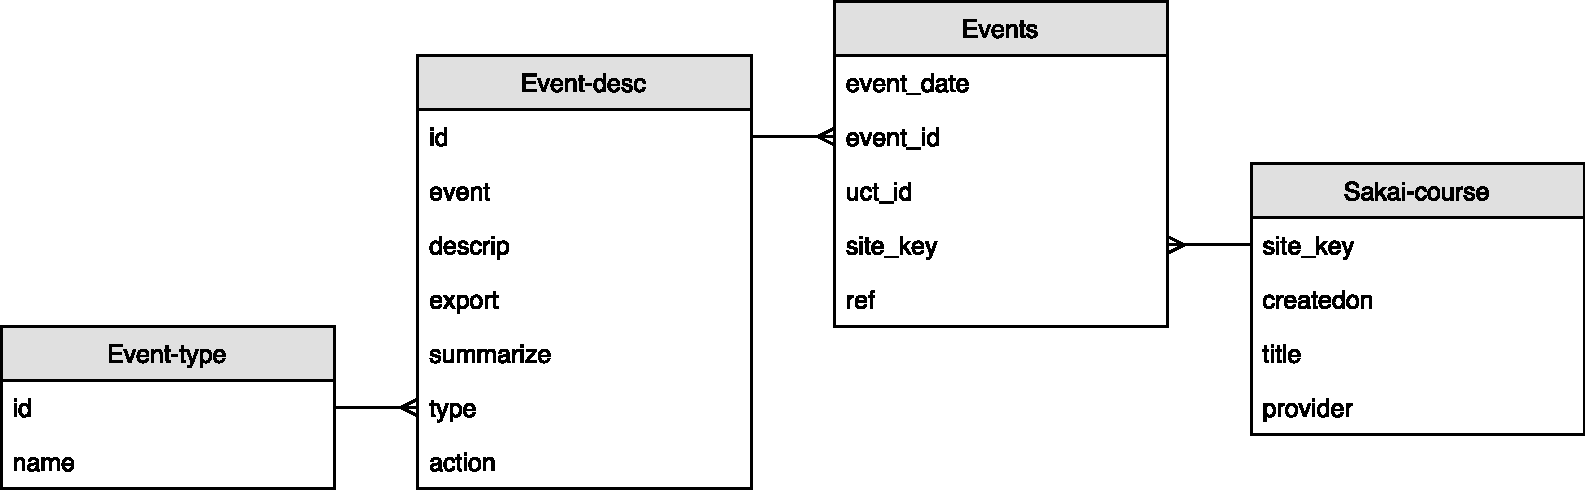
\includegraphics[scale=0.4]{./resources/figures/SakaiEvents}
  \caption[SakaiEventModel]{SakaiEventModel}
  \label{SakaiEventModel}
\end{figure}

\subsubsection*{Course Grades}
The course-grade entity export as used in this project is relatively simple - a flat CSV export with 26 columns, with \ref{Grades Columns} listing the fields that are used in this analysis. Further filtering is required on the \textit{RegCareer} field as shown in \ref{RegCareerFilter} and on course suffixes as shown in \ref{CourseSuffixFilter}. In addition, certain values of the \textit{Percent} attribute need to be scrubbed to normalize these values as numbers - a description of the logic used for this is shown in \ref{PercentTreatment}. Similarly to the event entity as mentioned above, an attribute has been added to each CSV row to identify the Course Grade entity within CouchDB. A resultant course grade in CouchDB looks like this:

\begin{minted}{json}
{
  "_id": "7530f4eed7e6bc3ef0d99a53be8ba9a2",
  "_rev": "8-232d0cf39728d41b4c5935f12469209d",
  "RegAcadYear": 2016,
  "RegTerm": 1161,
  "anonIDnew": 1,
  "RegCareer": "UGRD",
  "Degree": "QHB002",
  "Course": "PHI1010S",
  "CourseSuffix": "S",
  "Percent": "55",
  "CourseID": 109157,
  "Dept": "PHI",
  "type_": "courseGrade"
}
\end{minted}

\begin{table}[]
  \centering
  \caption{List of white-listed columns for the Course Grade entity: only these fields are used in the analysis.}
  \label{Grades Columns}
  \begin{tabular}{ll}
    Column Name  & Description                 \\ \hline
    RegAcadYear  & Year of course registration \\
    RegTerm      & Registration year ID        \\
    anonIDnew    & Student identification      \\
    RegCareer    & Undergrad or other          \\
    Degree       & Degree code                 \\
    Course       & Catalog ID                  \\
    CourseSuffix & Session information         \\
    Percent      & Grade achieved              \\
    CourseID     & Numerical ID                \\
    Dept         & Department                  \\
    CourseCount  & Course credit information   \\ \hline
  \end{tabular}
\end{table}

\begin{table}[]
  \centering
  \caption{RegCareer value list in terms of filtering}
  \label{RegCareerFilter}
  \begin{tabular}{ll}
    RegCareer & Included \\ \hline
    MAST      & FALSE    \\
    PDEV      & FALSE    \\
    BUSN      & FALSE    \\
    HONS      & FALSE    \\
    EMST      & FALSE    \\
    PGDP      & FALSE    \\
    UGRD      & TRUE     \\
    DOCT      & FALSE    \\
    NDGP      & FALSE    \\
    PDOC      & FALSE    \\
    MEDS      & FALSE    \\
    NDGU      & FALSE    \\ \hline
  \end{tabular}
\end{table}

\begin{table}[]
  \centering
  \caption{CourseSuffixFilter}
  \label{CourseSuffixFilter}
  \begin{tabular}{lll}
    Suffix & Include & Treatment \\ \hline
    D      & FALSE   & /         \\
    F      & TRUE    & S1        \\
    H      & TRUE    & S1 \& S2  \\
    L      & TRUE    & S1        \\
    M      & FALSE   & /         \\
    N      & FALSE   & /         \\
    P      & TRUE    & S2        \\
    Q      & FALSE   & /         \\
    R      & FALSE   & /         \\
    S      & TRUE    & S2        \\
    W      & TRUE    & S1 \& S2  \\
    X      & FALSE   & /         \\
    Z      & FALSE   & /         \\ \hline
  \end{tabular}
\end{table}

\begin{table}[]
  \centering
  \caption{Grade results need to be treated as numbers for the purpose of this analysis, this table shows all different value types and the appropriate treatment for each}
  \label{PercentTreatment}
  \begin{tabular}{lll}
    Symbol & Meaning                  & Handling Logic  \\ \hline
    49A    & Absent for supplementary & Grade used      \\
    49S    & Supplementary pending    & Grade used      \\
    50C    & ?                        & Grade used      \\
    78     & Grade                    & Grade used      \\
    AB     & Absent (fail)            & 40\% Grade used \\
    ATT    & ?                        & N/A             \\
    DE     & Deferred                 & N/A             \\
    DPR    & Duly performed refused   & 20\% Grade used \\
    F      & Fail                     & 40\% Grade used \\
    GIP    & Thesis only              & N/A             \\
    INC    & Incomplete (fail)        & 20\% Grade used \\
    LOA    & Leave of absence         & N/A             \\
    OS     & Outstanding              & N/A             \\
    OSS    & Outstanding              & N/A             \\
    PA     & Pass (thesis)            & N/A             \\
    SAT    & Thesis only              & N/A             \\
    UF     & Unclassified Fail        & 30\% Grade used \\
    UNS    & Thesis only              & N/A             \\
    UP     & Unclassified pass        & 50\% Grade used \\ \hline
  \end{tabular}
\end{table}